\documentclass[12pt,tikz]{instruction}
 

\begin{document} 
\begin{titlepage}
	\centering	
	\texttt {\moddate{\jobname.tex} v3.0}

	{\scshape\small Национальный исследовательский университет \\
		``Высшая школа экономики'' \par}
	\vspace{2cm}
	{\scshape\Large ``Система интеллектуальной \\кластеризации данных'' \\
		(Intelligent Data Clustering Toolkit, \SysName)\par}
	\vspace{1.5cm}
	{\Huge\bfseries ИНСТРУКЦИЯ ПОЛЬЗОВАТЕЛЯ\par}
	\vspace{2cm}
	\vfill
	\begin{center}
		\begin{tabular}{  p{7cm}  p{4cm} p{5cm}  } 
			& & \textbf{Разработчик:}\\ 
			& & Еремейкин П.А. \\ 
			& & студент группы \\
			& & мНоД16\_ТМСС\\
			& & \\
			& & \textbf{Руководитель: }\\
			& & профессор\\
			& & Миркин Б.Г.\\
		\end{tabular}
	\end{center}
	\vfill
	{Москва \the\year\par}
\end{titlepage}

%
%\begin{steps}
%	\begin{stept}{img2/norm-several.png}{Выбрать признаки для нормализации}
%		Для запуска нормализации нескольких признаков сразу, требуется нажать иконку 
\includegraphics[scale=0.1]{img2/norm_all.png}. Откроется окно выбора признаков. 	
%	\end{stept}
%	
%	\begin{stept}{img2/norm-several.png}{Выбрать признаки для нормализации}
%		В открытом окне выбрать те признаки, которые требуется нормализовать. По умолчанию отмечены признаки, которые не являются категориальными. Если требуется нормализовать в том числе категориальные, их следует отметить. Подтвердить выбор признаков, нажав кнопку \button{Ok}. Если имеется хотя бы один категориальный признак, то программа запросит подтверждение разложения признака по количеству уникальных значений. В случае согласия программа представит номинальный признак с помощью бинарных.
%	\end{stept}
%\end{steps}

\section*{Аннотация}
Система интеллектуальной кластеризации данных \SysName представляет собой программный комплекс, предназначенный для проведения кластер-анализа с применением интеллектуальных подходов. Задача кластер-анализа состоит в разделении таблицы объектов в множества (кластеры) таким образом, чтобы сходные объекты попали в один и тот же кластер, а несходные --- в разные. Широко известен традиционный метод \kmeans. Однако, этот метод обладает существенным недостатком: для его применения необходимо знать число кластеров, на которые будут разбиты данные. Для практического применения этот недостаток зачастую вынуждает отказаться от использования \kmeans. В этом случае задачу позволяют решить интеллектуальные методы, которые в процессе работы или другими способами позволяют автоматически определить число кластеров. Программная система \SysName обладает всем необходимым функционалом и включает в свой инструментарий множество методов, необходимых для решения сложных задач кластер анализа.
\newpage
	
\tableofcontents 

\newpage
\section{Введение}
\subsection{Область применения} 

Программное обеспечение \SysName применяется для проведения кластер-анализа таблиц данных с использованием интеллектуальных алгоритмов. Типичный пример задачи для решения который может применяться кластер-анализ --- задача об ирисах Фишера. Эта задача состоит в поиске 50 экземпляров каждого из трёх видов ириса --- Ирис щетинистый (Iris setosa), Ирис виргинский (Iris virginica) и Ирис разноцветный (Iris versicolor) на данных из 150 объектов. Каждый объект обладает четырьмя признаками: 
\begin{enumerate}
	\item Длина чашелистика
	\item Ширина чашелистика
	\item Длина лепестка
	\item Ширина лепестка
\end{enumerate}
Кластер-анализ применяется во многих областях, включая компьютерное зрение, маркетинг, биоинформатику и медицину\cite{amorim}.


\subsection{Описание возможностей} 
Программа \SysName предоставляет пользователю возможности просмотра таблиц данных, нормализации данных, кластер-анализа и визуализации результатов. Кроме того, возможности программы включают в себя генерацию искусственных данных. 

\subsection{Уровень подготовки пользователя}
Для работы с программой от пользователя требуется знание основ работы с графическим интерфейсом современных операционных систем (ОС).

\subsection{Исходный код}
Программа обладает открытым исходным кодом. Исходный код программы можно получить из github репозитория по следующим ссылкам:
\begin{enumerate}
	\item \url{https://github.com/eremeykin/ect} --- репозиторий с исходным кодом библиотек кластеризации (для вызова из \Python программ)
	\item \url{https://github.com/eremeykin/ectgui2} --- репозиторий с графической оболочкой, которая использует библиотеку кластеризации.
\end{enumerate}
Для запуска  интерфейса программы из исходных кодов потребуется выкачать оба репозитория. Если необходимо только использовать реализованные алгоритмы кластеризации, вызывая их из другой \Python программы, потребуется только первый репозиторий.

\section{Назначение}

Система интеллектуальной кластеризации \SysName предназначена для выделения из таблиц наблюдения множеств (кластеров) таким образом, чтобы сходные объекты попадали в один и тот же кластер, а несходные — в разные кластеры \cite{data-science}. Основной целью \SysName является повышение эффективности анализа данных. Функционалом системы предусмотрено два типа работ:
\begin{itemize}
	\item кластеризация реальных данных
	\item проведение численного эксперимента с синтетическими данными
\end{itemize}

\section{Условия применения и подготовка к работе}

Программный продукт работает в операционной системе Microsoft Windows 7 \footnote{Программная система разработана на кросплатформенном языке программирования \Python и может быть запущена также на других операционных системах, при условии удовлетворения всех необходимых зависимостей. Установка библиотек для различных OC выходит за рамки инструкции. Версия для Windows специально подготовлена для использования без необходимости установки интерпретатора или программных библиотек.} со следующими характеристиками:
\begin{itemize}
	\item объем ОЗУ не менее 2 Гб
	\item объем жесткого диска не менее 40 Гб
	\item микропроцессор с тактовой частотой не менее 1.5 Гц
	\item монитор с разрешением от $1280 \times 1024$ точек и выше
\end{itemize}

Все программные компоненты уже включены в распространяемый каталог, установка интерпретатора \Python и специальных библиотек не требуется. Необходимые dll библиотеки и другие ресурсы также  находятся в каталоге бинарных файлов в полном составе.
	
Для подготовки системы к работе требуется скопировать каталог с бинарными файлы программы с носителя на котором распространяется программа на запоминающее устройство ПК пользователя.  Каталог бинарных файлов назван \BinCatalog. Для начала работы пользователь запускает на выполнение файл \ExeFile из каталога бинарных файлов. При необходимости, пользователь может создать ярлык на исполняемый файл и запускать программу из любого удобного места. 

В каталоге бинарных файлов пользователь может также найти каталог \DataCatalog, в котором собраны некоторые иллюстративные наборы данных. Загрузка этих файлов в программу протестирована и не вызывает ошибок, поэтому их можно использовать для понимания структуры загружаемых файлов. Подробнее о требованиях к файлам данных см. раздел \fullref{subsec:trainfile}.

Настройки программа хранит в файле \SettingsFile. При необходимости, пользователь может удалить его, чтобы сбросить все настройки или изменять вручную (как правило, такой необходимости нет). 
 

\section{Основные приципы работы}

\subsection{Этапы работы с программой}
Работа с программой \SysName строится на основе графического диалогового интерфейса. Типичный сценарий взаимодействия пользователя с программой разделяется на следующие этапы:
\begin{enumerate}
	\item Запуск программы
	\item Загрузка исходных данных
	\item Нормализация
	\item Отбор признаков
	\item Выполнение кластеризации
	\item Просмотр результатов и текстового отчёта
\end{enumerate}

После запуска программы требуется выбрать файл, содержащий данные для кластеризации. Затем производится настройка параметров нормализации (см. \ref{subsec:norm}), отбор признаков, участвующих в кластеризации и выбор основных свойств применяемого алгоритма. После выбора необходимых параметров пользователь запускает алгоритм кластеризации. Когда выполнение кластеризации заканчивается, пользователю становятся доступны результаты работы для просмотра, анализа и сохранения. 

\subsection{Требования к файлу исходных данных}
\label{subsec:req}
Источником данных для программы является текстовый файл. Следует уделить особое внимание формату файла. Ниже перечислены требования к загружаемому файлу:
\begin{enumerate}
	\item Файл содержит записи в формате таблицы объект-признак
	\item Строки таблицы соответствуют объектам
	\item Столбцы таблицы соответствуют признакам
	\item Разделитель строк --- символ перевода строки (CR+LF для Windows)
	\item Разделитель столбцов --- запятая
	\item Первая строка обязательно содержит перечень названий признаков
	\item Названия признаков состоят только из латинских букв
	\item Разделитель дробной и целой части --- точка
	\item Значения номинальных признаков записываются в одно слово из латинских букв. Цифры не допустимы.
\end{enumerate}
Пример файла с  валидной структурой приведён в разделе \fullref{subsec:trainfile}.

\subsection{Обучающий файл}
\label{subsec:trainfile}

Демонстрация возможностей программы будет проиллюстрирована на обучающем наборе данных. Файл \SampleFile с демонстрационной таблицей данных можно найти в каталоге бинарных файлов программы в директории \DataCatalog. Этот файл можно открыть с помощью текстового редактора, например стандартного блокнота Windows и при необходимости отредактировать или просто посмотреть содержимое. 

Демонстрационный файл содержит таблицу параметров сматрфонов, продаваемых в магазине Ozon (\url{http://www.ozon.ru/}) в IV квартале 2017 года. Каждому смартфону соответствует 7 параметров: name, price, diag, cpu, ram, stype, vendor; соответственно название смартфона, цена в рублях, диагональ экрана в дюймах, частота процессора в ГГц, объем ОЗУ в Мб, тип матрицы, вендор.

Пример файла исходных данных, удовлетворяющий требованиям, описанным в разделе \fullref{subsec:req}, приведён ниже. Показаны только несколько первых строк, полный файл содержит 581 модель смартфона. Названия сокращены в целях наглядности.

\begin{tcolorbox}[colframe=black!50!black,coltext=black!25!black,colback=white,title=\textbf{Пример файла входных данных \SampleFile}]
	\verb|          name,      price,   diag,    cpu,    ram,   stype,   vendor |\\
	\verb|Meizu U10 32GB,   11990.00,    5.0,   1.50,   3072,     IPS,    Meizu |\\
	\verb|ZTE Blade A510,    7011.00,    5.0,   1.00,   1024,     IPS,      ZTE |\\
	\verb|Huawei P9 Lite,   14190.00,    5.2,   2.00,   2048,     IPS,   Huawei |\\
	\verb|Meizu M5 32GB ,   12990.00,    5.2,   1.50,   3072,     IPS,    Meizu |\\
	\verb|ZTE Blade L370,    4990.00,    5.0,   1.30,   1024,     TFT,      ZTE |\\
	\verb|BQ Aquaris M5 ,   18072.00,    5.5,   1.50,   3072,     IPS,       BQ |\\	
\end{tcolorbox}

\subsection{Нормализация}
\label{subsec:norm}
Нормализация --- это преобразование данных для приведения всех признаков к сопоставимым шкалам и началам отсчёта. Общая формула нормализации может быть записана следующим образом:
\begin{equation}\label{eq:normalization}
	X'=\dfrac{X-c}{r},
\end{equation}
\noindent где $X$ --- исходные данные,\\
\phantom{где\space}$c$ --- параметр, определяющий преобразование начала отсчёта,\\
\phantom{где\space}$r$ --- параметр, определяющий преобразование масштаба шкалы.

В некоторых случаях нормализация влияет существенным образом на результат кластеризации. 
В программе \SysName реализованы наиболее популярные способы определения параметра преобразования начала отсчёта:
\begin{itemize}
	\item среднее
	\item минимум
	\item медиана
	\item центр Минковского
\end{itemize}

Для параметра, определяющего разброс, предусмотрены следующие способы вычисления:
\begin{itemize}
	\item полуразмах
	\item стандартное отклонение
	\item абсолютное отклонение
\end{itemize}
 
В системе \SysName процедура нормализации реализована независимо от кластеризации и параметры нормализации могут быть изменены практически на любой стадии работы с системой. Как правило, нормализация задаётся сразу после загрузки исходных данных. Этап нормализации можно пропустить, если данные уже нормированы или в этом нет необходимости по мнению пользователя.

Выполнению кластеризации предшествует выбор параметров и принципов, на которых основывается процесс поиска однородных множеств. После выбора всех необходимых параметров пользователь производит запуск алгоритма и получает результат в интерфейсе программы. 

\subsection{Просмотр результатов кластеризации}

Просмотр результатов кластеризации может состоять в отслеживании принадлежности каждого объекта определенным кластерам или получении графического представления найденной кластерной структуры. Также система INDACT позволяет представить результат в виде интегральной таблице или в виде текстового отчёта.


\subsection{Общие сведения о пользовательском интерфейсе}

\subsubsection{Главное окно}
\label{subsec:gui}
Как было отмечено ранее, программа обладает графическим пользовательским интерфейсом. В данном разделе приведены основные сведения относительно элементов управления, их положения и функциях.

\begin{figure}[H]
	\begin{tikzpicture}
		\node[anchor=south west,inner sep=0] (image) at (0,0) {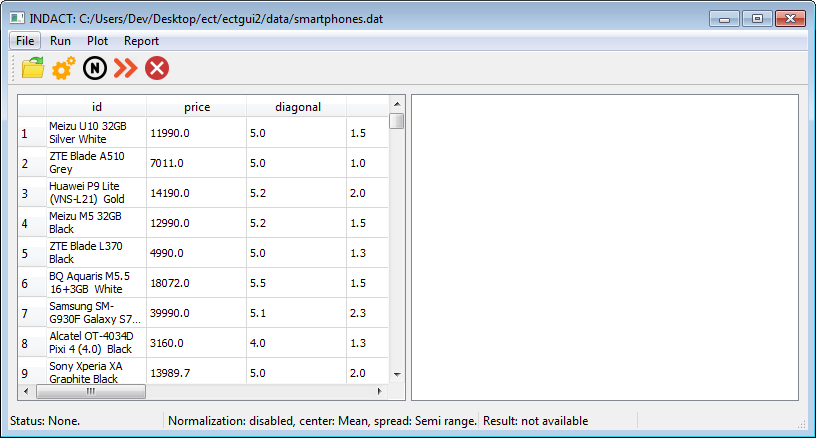
\includegraphics[width=0.8\textwidth]{img2/main-window.png}};
		\regnoter[thin](-1.4,6)(1:0.1:6.4);
		\regnoter[thin](-1,7.4)(2:0.4:6.4);
		\regnoteb[thin](0.6,8)(3:1:6.4);
		\regnoteb[thin](1.5,8.5)(4:1.5:6.4);
		\regnotel[thin](4.2,8.5)(5:2.2:6.4);
		\regnotel[thin](8.5,8)(6:6.:6.8);
		\regnoter[thin](10.3,8)(7:11.8:6.8);
		\regnoteb[thin](11.9,8)(8:12.3:6.8);
		\regnotel[thin](13.5,8)(9:12.8:6.8);
		\regnoter[thin](-1.4,4.4)(10:0.5:6);
		\regnoter[thin](-1.4,3.0)(11:1:6);
		\regnoteb[thin](2.5,8.5)(12:1.5:6);
		\regnotel[thin](4,7.5)(13:2.2:6);
		\regnoteb[thin](5.2,7.8)(14:2.7:6);
		\regnoter[thin](-1.4,1.6)(15:1:5.4);
		\regnoter[thin](-1.4,0.2)(16:0.5:2);
		\regnoter[thin](-1.4,-1.2)(17:0.5:0.2);
		\regnoter[thin](1.4,-1.2)(18:3:0.2);
		\regnoter[thin](6.,-1.2)(19:8:0.2);
		\regnote[thin](3,3.0)(20)
		\regnote[thin](10,3.0)(21)
		%\draw (-2,0) to[grid with coordinates] (18,10);
		\end{tikzpicture}
	\caption{Основные элементы пользовательского интерфейса}
	\label{fig:gui}
\end{figure}
Цифры на рисунке означают:
\begin{enumerate}
	\item Главное меню, элемент интерфейса, содержащий основные команды
	\item Меню File, содержит пункты:
		\begin{itemize}
			\item Load data file (\Ctrl + \texttt{O}) --- для загрузки файла данных
			\item Data operations --- для манипулирования данными
			\item Exit (\Ctrl + \texttt{Q}) --- для выхода из программы
		\end{itemize}
	\item Меню Run, содержит пункты для запуска соответствующих алгоритмов:
		\begin{itemize}
			\item \AWard (\Ctrl + \texttt{1})
			\item \AWardpb (\Ctrl + \texttt{2})
			\item \BiKMR (\Ctrl + \texttt{3})
			\item \dePDDP (\Ctrl + \texttt{4})
			\item \IKmeans (\Ctrl + \texttt{5})
		\end{itemize}
	\item Меню Plot, служит для вызова команд графического отображения, содержит пункты:
	\begin{itemize}
		\item By Markers --- для построения поля рассеяния (scatter plot) по отмеченным признакам
		\item SVD --- для построения SVD диаграммы 			
		\item Remove markers --- для удаления всех отметок признаков
	\end{itemize}
	

	\item Меню Report для формирования отчёта, содержит пункты:
		\begin{itemize}
			\item Text (\Ctrl + \texttt{R})--- для отображения текстового отчёта
			\item Text --- для отображения табличного отчёта
		\end{itemize}
	\item Заголовок окна, содержит путь к открытому файлу
	\item Кнопка ``Свернуть окно''
	\item Кнопка ``Развернуть окно''		
	\item Кнопка ``Закрыть окно''
	\item \label{itm:load-ico} Иконка ``Загрузить данные'', дублирует соответствующий пункт меню
	\item \label{itm:settings} Иконка ``Настройки'' вызывает диалог настроек нормализации
	\item \label{itm:norm-button} Иконка включения/выключения нормализации
	\item \label{itm:norm-several} Иконка нормализации нескольких признаков сразу
	\item \label{itm:delete} Иконка очистки нормализованных признаков
	\item Названия признаков
	\item Номера/названия объектов
	\item Строка состояния, выводит информацию о выполняемом действии
	\item Текущие параметры нормализации
	\item Последний результат кластеризации
	\item \label{itm:panel-raw} Панель с исходными данными 
	\item \label{itm:panel-norm} Панель с нормализованными данными 
\end{enumerate}

\subsubsection{Контекстное меню}
В данном разделе описаны пункты контекстного меню. Контекстное меню объединяет набор действий над определенным объектом и вызывается щелчком правой кнопки мыши на этом объекте. На рисунке \ref{fig:context-menu} показано контекстное меню для признака \texttt{price}.

\begin{figure}[h!]
	\centering
	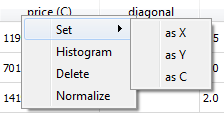
\includegraphics[width=0.35\textwidth]{img2/context-menu.png}
	\caption{Контекстное меню признака \texttt{price}}
	\label{fig:context-menu}
\end{figure}

Контекстное меню содержит следующие пункты:
\begin{enumerate}
	\item Set --- устанавливает особые свойства для признака (см. \ref{subsubsec:scatterplot}, \ref{subsubsec:asindex})
	\begin{enumerate}
		\item as X --- выставить метку \texttt{X} для признака (см. \ref{subsubsec:scatterplot})
		\item as Y --- выставить метку \texttt{Y} для признака
		\item as C --- выставить метку \texttt{C} для признака
		\item as Index (\texttt{TODO!}) --- установить признак как индекс (см. \ref{subsubsec:asindex})
	\end{enumerate}
	\item Histogram --- строит гистограмму по выбранному признаку (см. \ref{subsubsec:hist})
	\item Delete --- удаляет признак из вкладки, в которой вызвано контекстное меню (\mbox{см. \ref{subsubsec:deleteone}})
	\item Normalize --- нормализует выбранный признак, добавляя на панель нормализованных данных (см. \ref{subsubsec:onenorm})

	
\end{enumerate}

\newpage
\subsubsection{Диалог нормализации}

На рисунке \ref{fig:normdialog} показан диалог нормализации. Это окно требует от пользователя выставить значения для проведения нормализации (см. \ref{subsec:norm},\ref{sec:norm}). 
\begin{figure}[H]
	\centering
	\begin{tikzpicture}
	\node[anchor=south west,inner sep=0] (image) at (0,0) {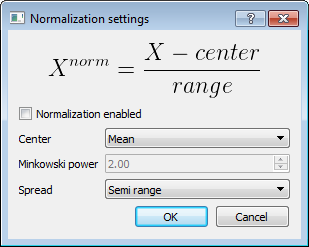
\includegraphics[width=0.45\textwidth]{img2/norm-dialog.png}};
	\regnoter[thin](-1.4,2.8)(1:0.6:3.2);
	\regnotel[thin](8,6.5)(2:6.9:5.5);
	\regnotel[thin](8,4.2)(3:6:4.2);
	\regnotel[thin](8,2.8)(4:6.5:2.6);
	\regnotel[thin](8,1.4)(5:6.5:2);
	\regnotel[thin](8,0.0)(6:6.5:1.4);
	
	\regnotel[thin](8,-1.4)(7:6.4:0.8);	
	\regnotel[thin](6,-1.4)(8:4.5:0.8);
	
%	\draw (-2,0) to[grid with coordinates] (18,10);
	\end{tikzpicture}
	\caption{Диалог установки параметров нормализации}
	\label{fig:normdialog}
\end{figure}
Цифры на рисунке означают:
\begin{enumerate}
	\item Переключатель вкл./выкл. нормализацию
	\item Кнопка закрытия окна
	\item Расчётная формула
	\item Выпадающий список для выбора центра нормализации
	\item Поле ввода степени Минковского (активно когда выбран центр Минковского)
	\item Выпадающий список для выбора диапазона нормализации
	\item Кнопка отмены
	\item Кнопка подтверждения ввода
\end{enumerate}

\subsubsection{Окно графического вывода}
\label{subsec:plot-view}
Окно графической информации служит для просмотра различного вида графиков и диаграмм. Такое окно может встретиться пользователю, например при построении гистограммы (раздел \ref{subsubsec:hist}), SVD диаграммы (\ref{subsubsec:svd}) или поля рассеяния (\ref{subsubsec:scatterplot}).

\begin{figure}[H]
	\centering
	\begin{tikzpicture}
	\node[anchor=south west,inner sep=0] (image) at (0,0) {	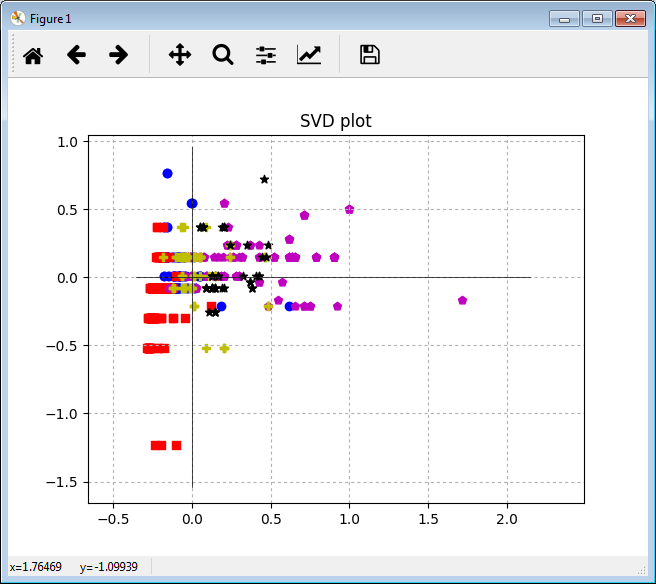
\includegraphics[width=0.5\textwidth]{img2/svd-plot.png}};
	\regnoter[thin]( -1.4 , 6.2)(1:0.4:6.6);
	\regnoter[thin]( -1   , 7.7)(2:1:6.6);
	\regnoteb[thin](  1.1 , 7.7)(3:1.5:6.6);
	\regnoteb[thin](  2.4 , 7.7)(4:2.3:6.6);
	\regnotel[thin](    4 , 7.7)(5:2.8:6.6);
	\regnotel[thin](  5.5 , 7.7)(6:4.7:6.6);
	\regnotel[thin](  9.2 , 7.7)(7:7.1:7.1);
	\regnotel[thin](  9.2 , 5.8)(8:7.9:7.1);
	\regnotel[thin](  9.2 , 4.4)(9:7.5:7.1);
	\regnotel[thin](  9.2 , 3.0)(10:7:5);
%	\draw (-2,0) to[grid with coordinates] (18,10);
	\end{tikzpicture}
	\caption{Окно графического вывода}
	\label{fig:plot-view}
\end{figure}


Цифры на рисунке означают:
\begin{enumerate}
	\item \label{itm:view-control1}Кнопка восстановления исходного автоматического положения и масштаба
	\item Кнопка возврата к предыдущему виду (после масштабирования или смещения)
	\item Кнопка возврата к следующему виду (после масштабирования или смещения)
	\item Кнопка смещения диаграммы
	\item Кнопка масштабирования выбранной области
	\item \label{itm:view-control6}Кнопка сохранения текущего графика в файл
	\item Свернуть окно
	\item Развернуть окно
	\item Закрыть окно 
	\item Изображение
\end{enumerate}

\subsubsection{Окно генерации данных}
Окно генерации применяется при работе с синтетическими данными (см. раздел \ref{subsec:generation}). Это окно необходимо для ввода информации о значениях характеристик генерируемых данных.

\begin{figure}[H]
	\centering
	\begin{tikzpicture}
	\node[anchor=south west,inner sep=0] (image) at (0,0) {	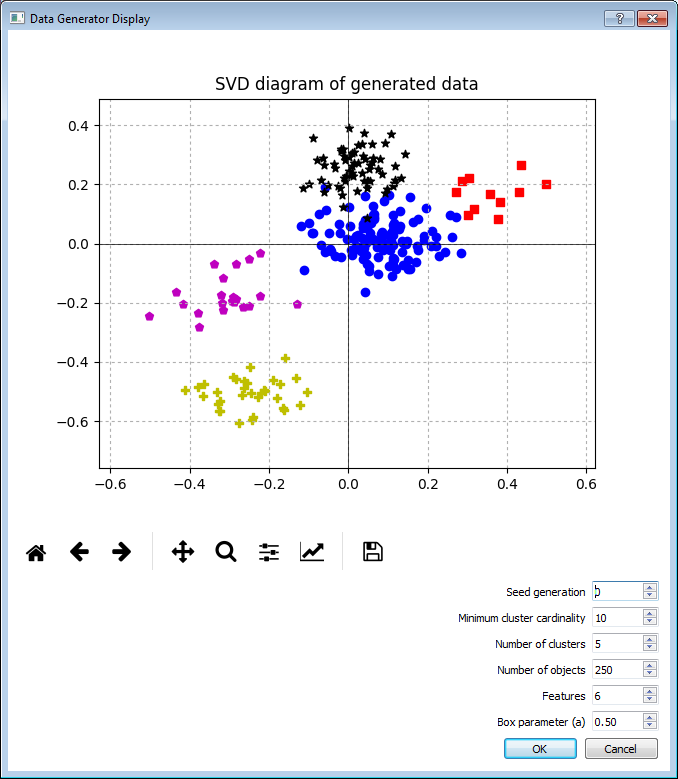
\includegraphics[width=0.8\textwidth]{img2/gen-data-dialog.png}};
	\regnotelmulti[thin](4,2)(1:0.8:4.2:1.6:4.2:2.5:4.2);
	\regnotel[thin](14,7)(2:9.4:10.7);
	\regnotel[thin](14,6)(3:12.4:3.7);
	\regnotel[thin](14,5)(4:12.4:3.1);
	\regnotel[thin](14,4)(5:12.4:2.6);
	\regnotel[thin](14,3)(6:12.4:2.1);
	\regnotel[thin](14,2)(7:12.4:1.6);
	\regnotel[thin](14,1)(8:12.4:1.1);
	\regnotel[thin](14,0)(9:12.4:0.6);
	\regnoter[thin](7,2)(10:10.4:0.6);
	
%	\regnotel[thin](13.5,-1.0)(7:13.5:1.3);
%	\draw (0,0) to[grid with coordinates] (18,10);
	\end{tikzpicture}
	\caption{Окно генерации данных}
	\label{fig:gen-data-dialog}
\end{figure}

Цифры на рисунке означают:
\begin{enumerate}
	\item Кнопки управления графиком (см. \ref{subsec:plot-view})
	\item Интерактивная графическая иллюстрация результата
	\item Поле ввода порождающего значения генератора (seed)
	\item Поле ввода минимального числа объектов в кластере
	\item Поле ввода числа кластеров
	\item Поле ввода числа объектов 
	\item Поле ввода числа признаков
	\item Поле ввода параметра смешения кластеров
	\item Кнопка отмены ввода
	\item Кнока подтверждения ввода
\end{enumerate}



\subsubsection{Окно запуска кластеризации}
\label{subsubsec:run-clustering-dialog}
В меню каждый алгоритм, реализованный в программе выделен отдельно. Для задания параметров алгоритма предусмотрены диалоговые окна. В данном разделе будут рассмотрены окна для настройки всех видов алгоритмов, реализованных в программе. 

\textbf{\AWard}

Окно для настройки параметров алгоритма \AWard изображено на рисунке \ref{fig:param-dialog-a-ward}.
\begin{figure}[H]
	\centering
	\begin{tikzpicture}
	\node[anchor=south west,inner sep=0] (image) at (0,0) {	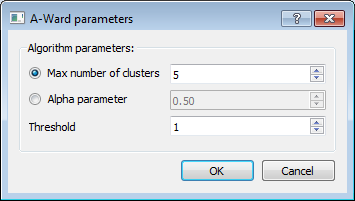
\includegraphics[width=0.45\textwidth]{img2/param-dialog-a-ward.png}};
	\regnotermulti[thin](-2,2)(1:0.7:2.1:0.7:2.7:0.7:2.7);
	\regnotel[thin](8,4)(2:6.2:2.6);
	\regnotel[thin](8,2.6)(3:6.2:2.2);
	\regnotel[thin](8,1.2)(4:6.2:1.6);
	\regnotel[thin](8,-0.2)(5:6.6:0.6);
	\regnotel[thin](6,-1.2)(6:4.5:0.6);
%	\draw (0,0) to[grid with coordinates] (18,10);
	\end{tikzpicture}
	\caption{Окно запуска \AWard}
	\label{fig:param-dialog-a-ward}
\end{figure}

Цифры на рисунке означают:
\begin{enumerate}
	\item Переключатель критерия остановки алгоритма
	\item Поле ввода максимального числа 
	\item Поле ввода параметра специального критерия
	\item Поле ввода порогового значения для отсечения небольших аномальных кластеров
	\item Кнопка отмены ввода
	\item Кнока подтверждения ввода
\end{enumerate}

\textbf{\AWardpb}

Для запуска алгоритма \AWardpb использутеся окно, показанное на рисунке \ref{fig:param-dialog-a-ward-pb}.

\begin{figure}[H]
	\centering
	\begin{tikzpicture}
	\node[anchor=south west,inner sep=0] (image) at (0,0) {	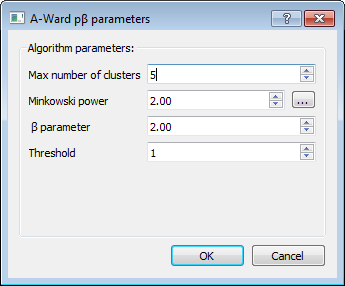
\includegraphics[width=0.45\textwidth]{img2/param-dialog-a-ward-pb.png}};
	\regnotel[thin](8,6)(1:6:4.6);
	\regnotel[thin](8,4.6)(2:5.4:4);
	\regnotel[thin](8,3.2)(3:6.5:4);
	\regnotel[thin](8,1.8)(4:6:3.4);
	\regnotel[thin](8,0.4)(5:6:2.8);
	
	\regnotel[thin](8,-1.0)(6:6.6:0.6);
	\regnotel[thin](6,-1.2)(7:4.5:0.6);
%	\draw (0,0) to[grid with coordinates] (18,10);
	\end{tikzpicture}
	\caption{Окно запуска \AWardpb}
	\label{fig:param-dialog-a-ward-pb}
\end{figure}

Цифры на рисунке означают:
\begin{enumerate}
	\item Поле ввода максимального числа кластеров
	\item Поле ввода степени Минковского
	\item Кнопка для запуска автоматического подбора степени Минковского
	\item Поле ввода степени весов признаков $ \beta $
	\item Поле ввода порогового значения для отсечения небольших аномальных кластеров
	\item Кнопка отмены ввода
	\item Кнока подтверждения ввода
\end{enumerate}

\textbf{\BiKMR}

Для запуска алгоритма \BiKMR требуется ввод всего одного параметра, соответствующее окно показано на рисунке \ref{fig:param-dialog-bikmr}.

\begin{figure}[H]
	\centering
	\begin{tikzpicture}
	\node[anchor=south west,inner sep=0] (image) at (0,0) {	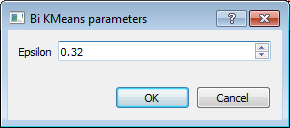
\includegraphics[width=0.4\textwidth]{img2/param-dialog-bikmr.png}};
	\regnotel[thin](7.5,2.5)(1:5.5:1.8);
	\regnotel[thin](6.5,-1.2)(2:5.6:0.6);
	\regnotel[thin](4.5,-1.2)(3:3.5:0.6);
%	\draw (0,0) to[grid with coordinates] (18,10);
	\end{tikzpicture}
	\caption{Окно запуска \BiKMR}
	\label{fig:param-dialog-bikmr}
\end{figure}

Цифры на рисунке означают:
\begin{enumerate}
	\item Поле ввода параметра $ \epsilon $
	\item Кнопка отмены ввода
	\item Кнока подтверждения ввода
\end{enumerate}

\textbf{\dePDDP}

Для запуска алгоритма \dePDDP не требуется вводить никаких параметров, он запускается сразу же после выбора соответствующего пункта меню.

\textbf{\IKmeans}

Окно запуска алгоритма \IKmeans такое же как и для \AWard.


\subsubsection{Окно таблицы результатов}
В программе результат кластеризации может быть представлен в табличном виде или в виде текстового отчёта.  Эти окна могут быть открыты только после выполнения одного из алгоритмов кластеризации. Окно табличного представления информации о полученных кластерах изображено на рисунке \ref{fig:table-report}. Значение в таблице соответствует среднему значению данного признака в данном кластере. Если это значение существенно больше общего среднего по признаку, то ячейка выделяется красным цветом, если существенно меньше --- синим.

\begin{figure}[H]
	\centering
	\begin{tikzpicture}
	\node[anchor=south west,inner sep=0] (image) at (0,0) {	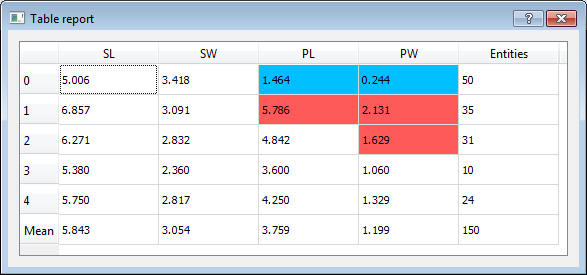
\includegraphics[width=0.6\textwidth]{img2/table-report.png}};
	\regnotermulti[thin](-1.5,2.5)(1:0.6:3.4:0.6:1.8:0.6:1.8);
	\regnotelmulti[thin](4,5.2)(2:1.8:3.8:3.5:3.8:3.5:3.8);
	\regnoter[thin](-1.5,1.1)(3:0.6:0.8);
	\regnoter[thin](6,5.2)(4:8.6:3.8);
%	\draw (0,0) to[grid with coordinates] (10,6);
	\end{tikzpicture}
	\caption{Окно табличного отчёта}
	\label{fig:table-report}
\end{figure}


Цифры на рисунке означают:
\begin{enumerate}
	\item Названия признаков
	\item Номера кластеров
	\item Строка средних значений по всем данным
	\item Столбец числа объектов в кластере
\end{enumerate}
Рисунок \ref{fig:text-report} изображает окно текстового отчёта, которое содержит единственный элемент для просмотра текста.
\begin{figure}[H]
	\centering
	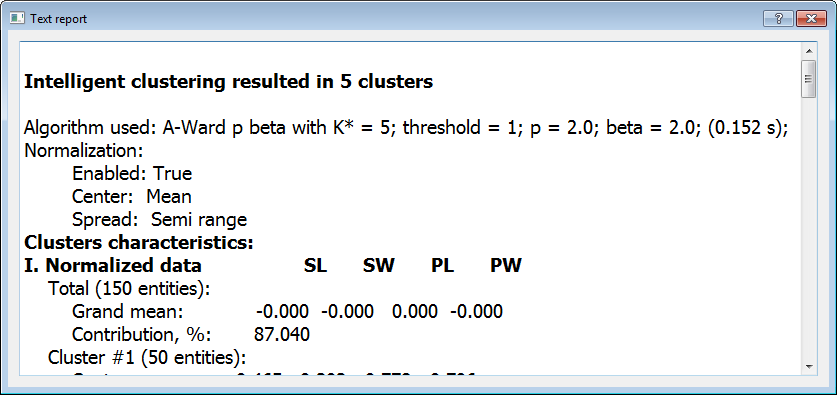
\includegraphics[width=0.6\textwidth]{img2/text-report.png}
	\caption{Окно текстового отчёта}
	\label{fig:text-report}
\end{figure}

\newpage
\section{Описание операций}

\subsection{Запуск программы}
Для работы с программой требуется запустить процесс OC, который отображает графический интерфейс и взаимодействует с пользователем. Действия этой операции приведены в таблице ниже.

\begin{steps}
	\begin{ist}{img2/run-exe.png}{Запустить бинарный файл программы}
		Дважды нажать левой кнопкой мыши (ЛКМ) на значке \texttt{INDACT.exe}
	\end{ist}
	\begin{ist}{img2/empty-window.png}{Дождаться запуска}
		Подождать, пока произойдёт инициализация среды выполнения Python. Открытие чёрного консольного окна, означает что установлена отладочная версия программы. Его не следует закрывать. Запуск программы занимает не более 3-4 сек.   
	\end{ist}
\end{steps}
	
\newpage
\subsection{Загрузка исходных данных}
\label{subsec:dataload}

Загрузка данных необходима для того, чтобы подать программе файл, который содержит таблицу данных. Формат файла должен удовлетворять набору требований, перечисленных в разделе \fullref{subsec:req}. 

\begin{steps}
	\begin{ist}{img2/open-file-menu.png}{Открыть диалог загрузки файла}
		Для открытия диалога загрузки файла необходимо последовательно нажать в главном меню пункты \menu{File} $ \Rightarrow $ \menu{Load data file}. Того же результата можно достичь нажатием иконки 
\includegraphics[scale=0.05]{img2/folder-ico.png} (см. рисунок \ref{fig:gui} обозначение \ref{itm:load-ico})
	\end{ist}
	
	\begin{ist}{img2/open-smartphones.png}{Выбрать текстовый файл с данными}
		В стандартном файловом диалоге необходимо выбрать загружаемый файл и нажать кнопку \button{Open}. Например, для загрузки демонстрационного примера следует выбрать файл \texttt{INDACT/data/} \SampleFile 
	\end{ist}
	\begin{ist}{img2/load-result.png}{Проверить загрузку исходного файла}
		После выполнения предыдущего пункта будет произведена загрузка файла и отображение его содержимого в виде таблицы в интерфейсе программы. Пользователю следует убедиться, что загружен правильный файл, объекты и признаки отображаются верно. На рисунке справа показан загруженный файл \texttt{smartphones.dat} 
	\end{ist}
\end{steps}


\subsection{Нормализация}
\label{sec:norm}
\subsubsection{Установка параметров нормализации}

Назначение и параметры нормализации описаны в разделе \fullref{subsec:norm}, примеры установки различных настроек нормализации описаны в разделе \ref{subsubseq:example_norm1}.
\begin{steps}
	\begin{ist}{img2/click-norm.png}{Открыть диалог нормализации}
		Диалог нормализации можно открыть щелчком ЛКМ на иконке 
\includegraphics[scale=0.1]{img2/settings.png} (см. рисунок \ref{fig:gui} обозначение \ref{itm:settings})
	\end{ist}
	\begin{ist}{img2/norm-settings-dialog.png}{Включить нормализацию}
		Чтобы включить нормализацию, требуется установить флажок ``\texttt{Normalization enabled}'' в открывшемся окне настроек нормализации.
	\end{ist}
	\begin{ist}{img2/norm-settings-dialog-edit.png}{Выставить параметры}
		Для нормализации данных необходимо задать центр и диапазон нормализации. Эти параметры выбираются из выпадающих списков. Нажать \button{Ok}.
	\end{ist}
	\begin{ist}{img2/norm-button-enabled.png}{Убедиться что нормализация включена}
		После применения настроек нормализации следует убедиться, что кнопка нормализации успешно включилась (см. рисунок \ref{fig:gui} обозначение \ref{itm:norm-button}).	
	\end{ist}	
\end{steps}

\newpage
\subsubsection{Нормализация одного признака}
\label{subsubsec:onenorm}
После настройки параметров нормализации необходимо выбрать какие признаки требуется нормализовать. Только выбранные признаки будут участвовать в кластеризации. В программе предусмотрено четыре возможности для выбора признаков: выбор по одному, выбор нескольких сразу и удаление по одному или сразу нескольких. 

\begin{steps}
	\begin{ist}{img2/norm-one-feature.png}{Выбрать признак для нормализации}
		Для выбора одного признака необходимо найти столбец признака на панели исходных данных (рисунок \ref{fig:gui} обозначение 	\ref{itm:panel-raw}) и нажать на нем правой кнопкой мыши (ПКМ). В контекстном меню выбрать пункт \menu{Normalize}. На примере показана операция нормализации признака \texttt{stype}.
	\end{ist}
	
	\begin{ist}{img2/norm-one-approve.png}{(При необходимости) Подтвердить нормализацию категориального признака}
		Если был выбран категориальный признак (в примере \texttt{stype}), то программа запросит подтверждение разложения признака на бинарные. В случае согласия произойдёт добавление бинарных признаков, отвечающих за наличие каждого из значений категориального признака \textit{ и их нормализация}.
	\end{ist}
		
	\begin{ist}{img2/norm-one-done-dual.png}{Просмотр вида таблицы}
		После выбора признака, он будет перенесён из вкладки на панель нормализованных данных и к нему будут применены выбранные настройки нормализации. Дополнительно на панели нормализованных данных будет отображён столбец ``\texttt{Cluster\#}'', который будет оставаться заполненным символами ``\texttt{?}'' до тех пор, пока не будет выполнен шаг кластеризации (см. верхний рисунок, нормализация признака \texttt{rom}). Сказанное выше справедливо и для номинального признака (например \texttt{stype}), но стоит иметь в виду что соответствующие бинарные признаки будут названы \texttt{stype[значение признака]} (как показано на нижнем рисунке)
	\end{ist}
		
\end{steps}

\newpage
\subsubsection{Нормализация нескольких признаков сразу}

Если признаков много и нормализовать их по одному долго, то можно воспользоваться функцией нормализации нескольких признаков сразу.

\begin{steps}
	\begin{ist}{img2/norm-several.png}{Запустить нормализацию нескольких признаков }
		Для запуска нормализации нескольких признаков сразу, требуется нажать иконку 
\includegraphics[scale=0.1]{img2/norm_all.png}. Откроется окно выбора признаков.
	\end{ist}
	\begin{ist}{img2/select-features-dialog.png}{Выбрать признаки для нормализации}
		В открытом окне выбрать те признаки, которые требуется нормализовать. По умолчанию отмечены признаки, которые не являются категориальными. Если требуется нормализовать в том числе категориальные, их следует отметить. Подтвердить выбор признаков, нажав кнопку \button{Ok}. Если имеется хотя бы один категориальный признак, то программа запросит подтверждение разложения признака по количеству уникальных значений. В случае согласия программа представит номинальный признак с помощью бинарных.
	\end{ist}		
	\begin{ist}{img2/norm-several-result.png}{Посмотреть результат}
		После нормализации признаков результат будет отображен на панели нормализованных данных (см. рисунок \ref{fig:gui}, обозначение \ref{itm:panel-norm})
	\end{ist}
		
\end{steps}



\newpage
\subsection{Отбор признаков}
\subsubsection{Удаление одного признака}
\label{subsubsec:deleteone}

Как было отмечено выше, программа позволяет удалять отдельные признаки из как c панели нормализованных данных, так и с панели исходных данных. Эта функция может быть применена для исключения из рассмотрения определённых признаков.

\begin{steps}
	\begin{ist}{img2/select-to-delete.png}{Выбрать признак для удаления}
		Для удаления одного признака необходимо найти столбец признака в нужной вкладке и нажать на нём ПКМ. В контекстном меню выбрать пункт \menu{Delete}. Рассмотрим удаление на примере признака \texttt{vendor}. Контекстное меню, открытое после нажатия на заголовке \texttt{vendor} показано на рисунке справа.
	\end{ist}
	\begin{ist}{img2/delete-one-result.png}{Посмотреть результат}
		В результате выполнения операции выбранный признак будет удалён только из панели исходных данных, но останется на второй панели.
	\end{ist}		
\end{steps}

\newpage
\subsubsection{Удаление нескольких признаков сразу}

Если требуется полностью очистить панель нормализованных данных или удалить большое количество признаков, то следует воспользоваться функцией, описанной ниже. Функция удаления нескольких признаков сразу может быть использована для быстрого исключения лишних признаков.

\begin{steps}
	\begin{ist}{img2/press-delete-ico.png}{Запустить удаление}
		Функция удаления нескольких признаков вызывается щелчком ЛКМ на иконке 
\includegraphics[scale=0.1]{img2/delete.png} (см. рисунок \ref{fig:gui} обозначение \ref{itm:delete}).
	\end{ist}
	\begin{ist}{img2/delete-several-select.png}{Выбрать удаляемые признаки}
		Выбор удаляемых признаков производится при помощи выставления соответствующих флажков. Все отмеченные признаки будут удалены из панели нормализованных данных. Когда выбор завершён, нажать кнопку \button{Ok}.
	\end{ist}	
	\begin{ist}{img2/delete-several-result.png}{Посмотреть результат}
		В результате выполнения операции выбранные признаки будут удалены с панели нормализованных данных.
	\end{ist}	
		
\end{steps}

\newpage
\subsection{Визуализация}
\subsubsection{Построение гистограммы признака}
\label{subsubsec:hist}

В качестве первичного инструмента анализа программа предлагает возможность построения гистограмм выбранного признака.

\begin{steps}
	\begin{ist}{img2/hist-pick-menu.png}{Выбрать признак}
		Для построения гистограммы необходимо определиться с признаком, по которому будет построена гистограмма. Для этого надо щёлкнуть ПКМ на названии столбца соответствующего признака. В контекстном меню выбрать пункт \menu{Histogram}. На примере показано построение гистограммы по признаку \texttt{price}
	\end{ist}
	\begin{ist}{img2/hist-set-bins.png}{Отрегулировать количество бинов}
		Как известно, вид гистограммы может зависеть от числа интервалов, на которые разбиваются область допустимых значений. Поэтому, в программе предусмотрена регулировка этого параметра. В нижнем полк ввода можно выставить требуемое число интервалов.
	\end{ist}
	\begin{ist}{img2/hist-result.png}{Посмотреть результат}
		Результат построения гистограммы будет доступен сразу же в том же окне. На рисунке справа показана гистограмма, построенная для ненормализованного признака \texttt{price} при количестве интервалов, равным 100. Окно отображения гистограммы обладает всеми стандартными кнопками для управления визуализациями, в том числе для сохранения в файл.
	\end{ist}		
\end{steps}	


\newpage
\subsubsection{Построение поля рассеяния (scatter plot)}
\label{subsubsec:scatterplot}

Для первичного анализа структуры данных или результатов кластеризации в программе предусмотрена функция построения поля рассеяния по меткам на выбранных признаках. Метка --- вспомогательный символ, присваиваемый пользователем для  определённого признака.  Предусмотрено 3 вида меток: ``\texttt{X}'', ``\texttt{Y}'', ``\texttt{C}''. Первый вид означает что отмеченный признак будет соответствовать координатам объекта по оси абсцисс, второй --- по оси ординат, а третий, что цвет (\textit{Color}) точки будет выбираться в соответствии со значением отмеченного признака

\begin{steps}
	\begin{ist}{img2/set-as-x.png}{Выбрать признак по оси X}
		Для построения поля рассеяния требуется задать признаки по осям абсцисс и ординат. Чтобы отметить признак, соответствующий оси абсцисс, требуется нажать на его названии ПКМ и в контекстном меню выбрать
		\menu{Set} $\Rightarrow$ \menu{as X}
	\end{ist}
	\begin{ist}{img2/set-as-x-done.png}{Посмотреть результат}
		После установки маркера ``\texttt{X}'' к имени соответствующего признак добавиться ``\texttt{(X)}''. На примере показано добавление метки ``\texttt{X}''  к признаку \texttt{diag}.
	\end{ist}	
	\begin{ist}{img2/set-as-y-done.png}{Выбрать признак по оси Y}
		Аналогично пунктам 1,2. В примере указан признак \texttt{cpu}.
	\end{ist}
	\begin{ist}{img2/set-as-c-done.png}{Выбрать признак, отвечающий за цвет (опционально)}
		Для того чтобы задать, какой признак будет определять цвет точек на диаграмме, необходимо выставить маркер ``\texttt{C}''. Для этого выбрать в контекстном меню выбрать \menu{Set} $\Rightarrow$ \menu{as С}. 
	\end{ist}
	\begin{ist}{img2/plot-by-markers.png}{Построить scater plot}
		В главном меню выбрать \menubox{\texttt{Plot}} $\Rightarrow$ \menubox{\texttt{By markers}} 
	\end{ist}
	\begin{ist}{img2/plot-by-markers-result.png}{Посмотреть результат}
		В новом окне откроется построенная красивая и цветастая диаграмма. Как и прочие окна отображения графической информации, окно отображения scatter plot имеет кнопки для управления видом и сохранения изображения в файл (подробнее см. рисунок \ref{fig:plot-view}, обозначения \ref{itm:view-control1}-\ref{itm:view-control6}). На примере показана диаграмма, у которой по оси X отложен признак \texttt{diag}, по оси Y --- \texttt{cpu}, цвет определяется признаком \texttt{stype}.
	\end{ist}
	\begin{ist}{img2/plot-by-markers-delete.png}{Удалить метки (опционально)}
		В главном меню выбрать \menubox{\texttt{Plot}} $\Rightarrow$ \menubox{\texttt{Delete All Markers}}. При этом отметки ``\texttt{X}'', ``\texttt{Y}'' и ``\texttt{C}'' будут удалены.
	\end{ist}
	
\end{steps}

\newpage
\subsubsection{Построение SVD диаграммы}
\label{subsubsec:svd}
Для интегральной оценки структуры данных предусмотрена функция построения SVD диаграммы. Имеется возможность построения SVD диаграммы по нормализованным и не нормализованным данным.
\begin{steps}
	\begin{ist}{img2/plot-svd.png}{Построить SVD диаграмму}
		Для построения SVD диаграммы в главном меню выбрать \menu{Plot} $\Rightarrow$ \menu{SVD} $\Rightarrow$ \menu{Normalized} или \menu{Raw} для построения диаграммы по нормализованным и не нормализованным данным соответственно.
	\end{ist}

	\begin{ist}{img2/svd.png}{Посмотреть результат}
		Построенная диаграмма откроется в новом окне, как показано на рисунке справа.\vspace{6.5cm}
	\end{ist}
\end{steps}

\subsection{Генерация синтетических данных}
\label{subsec:generation}
Для генерирования искусственных данных необходимо вызвать диалог настройки параметров, указать все необходимые величины и сохранить сгенерированные данные в файл.

\begin{steps}
	\begin{ist}{img2/gen-open-dialog.png}{Открыть диалог генерации данных}
		Чтобы открыть диалог загрузки данных, необходимо в главном меню программы выбрать \menu{File} $\Rightarrow$ \menu{Data operations} $\Rightarrow$ \menu{Generate}.
	\end{ist}
	\begin{ist}{img2/gen-dialog.png}{Указать параметры данных}
		В открывшемся диалоге необходимо указать параметры данных, по которым будет производиться генерация. Подробнее о параметрах генерации см. \cite{kovaleva}. В верхней части диалога отображается динамическая информирующая диаграмма. Когда все параметры будут введены, нажать кнопку \button{OK}. \vspace{1.2cm}
	\end{ist}
	\begin{ist}{img2/save-dataset.png}{Указать имя файла}
		В файловом диалоге указать имя файла, куда будут сохранены сгенерированные данные. Нажать кнопку \button{Ok} 
	\end{ist}
	\begin{ist}{img2/save-dataset-labels.png}{Выбрать как сохранить кластеры}
		Принадлежность кластера определяется по целочисленными меткам, присвоенным каждому объекту. Для задания способа сохранения меток откроется окно, как показано на рисунке справа. На выбор доступны опции сохранения меток как отдельный признак в том же файле, в отдельном файле или их можно вообще не сохранять. Выбрав нужную опцию, нажать \button{Ok}. Файлы будут сохранены соответственно выбранным настройкам.
	\end{ist}
\end{steps}

\newpage
\subsection{Запуск кластеризации}

Для определения принадлежности объектов кластерам требуется установить параметры кластеризации и запустить алгоритм.

\begin{steps}
	\begin{ist}{img2/run-clustering.png}{Открыть диалог выбора параметров}
		Для запуска алогритма кластеризации первым делом тербуется открыть диалого настройки параметров. Для этого выбрать в главном меню \menu{Run} $\Rightarrow$ \menu{<Алгоритм>}, где \texttt{<Алгоритм>} соответствует названию одного из реализованных алгоритмов, например, \AWard. Список всех реализованных алгоритмов можно увидеть на рисунке.
	\end{ist}
	\begin{ist}{img2/a-ward-dialog.png}{Настроить параметры алгоритма}
		Для большинства алгоритмов требуется указать некоторые управлящие параметры, для справки по соответствующим диалоговым окнам см. раздел. \fullref{subsubsec:run-clustering-dialog}. После задания параметров нажать кнопку \button{Ok}.
	\end{ist}
	\begin{ist}{img2/clustering-complete.png}{Дождаться результатов кластеризации}
		Сразу после нажатия кнопки \button{Ok} будет запущена работа алгоритма.
		Когда кластеризация будет завершена, в строке состояния будет выведена краткая информация о алгоритме и времени работы. В то же время в столбце \texttt{Cluster \#} будут проставлены метки кластеров. Каждая метка соответствует номеру кластера, которому принадлежит объект.
	\end{ist}
		
\end{steps}

\subsection{Генерация отчёта}
\label{subsec:report}
Результаты кластеризации удобно анализировать по сгенерированному отчёту. Программа \SysName предлагает два вида отчёта: текстовый и табличный.

\subsubsection{Текстовый отчёт}
\begin{steps}
	\begin{ist}{img2/report-text.png}{Сгенерировать отчёт}
		Для генерации текстового отчёта в главном меню выбрать \menu{Report} $\Rightarrow$ \menu{Text}.
	\end{ist}
	\begin{ist}{img2/select-features-dialog.png}{Выбрать признаки}
		Выбрать признаки, которые будут включены в текстовый отчёт. Для этого отметить флажки соответствующие тем признакам, которые требуется указать в отчёте. \vspace{2.5cm}
	\end{ist}
	
	\begin{ist}{img2/text-report-done.png}{Посмотреть окно отчёта}
		Окно текстового отчёта показано на рисунке справа и содержит только текстовое поле с табулированным отчётом. Из этого окна текст можно скопировать в файл.
	\end{ist}
		
\end{steps}

\newpage
\subsubsection{Табличный отчёт}

\begin{steps}
	\begin{ist}{img2/report-text.png}{Сгенерировать отчёт}
		Для генерации табличного отчёта в главном меню выбрать \menu{Report} $\Rightarrow$ \menu{Table}.
	\end{ist}
	\begin{ist}{img2/table-report-done.png}{Посмотреть окно отчёта}
		В окне табличного отчёта приведена сводная таблица в которой строки соответствуют кластерам, а столбцы --- признакам. В ячейках указаны средние значения признака по кластеру. Красным цветом выделены ячейки, в которых относительная разность значения и средней величины признака по кластеру больше 30\%, соответственно синим --- меньше 30\%. Маргинальная строка содержит средние значения признаков по всем кластерам, а столбец --- число объектов в кластере.
	\end{ist}
	
\end{steps}


\newpage
\subsection{Выход из программы}

\begin{steps}
	\begin{ist}{img2/exit-indact.png}{Выйти из программы}
			Для выхода из программы в главном меню выбрать \menu{File} $\Rightarrow$ \menu{Exit}. \textbf{Поздравляем, вы завершили работу с программой!}
	\end{ist}
\end{steps}

\section{Алгоритмы кластеризации (краткое описание)}
\label{sec:algs}
\subsection{Алгоритм  \AWard}
\label{subsec:a-ward}
Алгоритм \AWard является усовершенствованием  широко известного алгоритма иерархической агломеративной кластеризации Уорда (\Ward)\cite{ward}. На первом шаге все кластеры состоят из единственного объекта. 

Остановка алгоритма происходит при достижении числа кластеров, заданного пользователем, или объединении всех объектов в едином универсальном кластере. Степень близости между двумя кластерами вычисляется как произведение квадрата евклидовского расстояния между центрами кластеров и произведения численностей этих кластеров, делённого на их суммарную численность. 

Недостаток алгоритма Уорда --- медленность вычислений, связанная с необходимостью отыскания минимума расстояний, которых очень много на начальных этапах агломерации. В алгоритме А-Уорд эти шаги пропускаются, поскольку шаги агломерации применяются к некоторому предварительному разбиению объектов на достаточно малое число кластеров. Это-то предварительное разбиение используется как начальное для работы метода Уорда. Классы предварительного разбиения --- это кластеры, полученные методом аномальной кластеризации.

Метод аномальной кластеризации находит и удаляет аномальные кластеры по одному до тех пор, пока не останется объектов для кластеризации. В основе этого метода лежит критерий квадратичной ошибки метода к-средних. Аномальным называется такой кластер, который наиболее удалён от начала координат, куда предварительно переносится центр данных. Его построение начинается с самого удалённого объекта, а затем в него добавляются все объекты, которые ближе к центру кластера, чем к точке начала отсчёта. Центр аномального кластера обновляется на каждом шаге, в то время как центр данных остаётся неизменным.


\subsection{Алгоритм  \AWardpb}
Алгоритм \AWardpb --- это дополнительная модификация для приложений, в которых требуется анализировать зашумленные данные, включающие нерелевантные признаки. В этом случае и \Ward, и \AWard плохо работают. Снизить влияние нерелеFвантных признаков позволяет введение весовых коэффициентов. В процессе работы алгоритма \AWardpb для каждого признака вычисляется вес, обратно пропорциональный его разбросу  внутри кластера. При этом используется не обязательно евклидово расстояние, а метрика Минковского произвольной степени. Параметры $ p $ и  $ \beta $ являются степенями Минковского и 
весовых коэффициентов признаков соответственно.

Как и в случае с \AWard, алгоритм \AWardpb использует аномальную кластеризацию для предварительной ``разведки'' структуры данных и снижения времени работы, однако в алгоритме \AWardpb аномальная кластеризация обобщена с учётом дополнительных параметров.

\subsection{Алгоритм BiKM-R} 
Алгоритм BiKM-R (bisecting k-means randomized / Раздвоение по методу k-средних) относится к классу дивизивных алгоритмов иерархического кластер-анализа. В отличие от агломеративных алгоритмов, где вычисления организованы ``снизу-вверх'' путём объединения, здесь вычисления организованы ``сверху-вниз'' путём разделения кластеров, начиная с универсального кластера, состоящего из всех объектов. На каждом шаге определённый кластер S разбивается на два по критерию  суммы квадратов ошибок. Для инициализации алгоритма требуется указать начальные центры $c_1$ и $c_2$. Затем осуществляются двухшаговые итерации по методу к-средних при $ k=2 $. На первом шаге обновляются кластеры, путём разделения объектов на тех, что ближе к $c_1$ ( кластер $ S_1 $ ) и тех, что ближе к $c_2$ (кластер $ S_2$). На втором шаге вычисляются новые центры $ S_1 $ и $ S_2 $. Процесс заканчивается, как только новые центры совпадают со старыми. Как и в случае с агломеративным алгоритмом, выбор $c_1$ и $c_2$ может быть организован с использованием метода аномальных кластеров. Для инициализации алгоритма раздвоения используются центры двух наибольших аномальных кластеров.

Для остановки алгоритма BiKM-R используется критерий, основанный на проецировании точек 
кластеров на случайные направления. Пусть на некотором этапе работы алгоритма имеется K кластеров. Генерируются s случайных векторов $p_i$, $i=1,\ldots,s$. Для генерации используется нормальное 
сферическое распределение со средним в начале координат и $\sigma^2=1/V$, где $V$ – количество признаков. 
Затем каждый элемент $x$ каждого кластера $S_k$ ($k=1,\ldots, K$) проецируется на направления $p_i$, 
координаты проекции определяются как скалярное произведение: $x_i=<x,p_i>$. Для каждого направления 
вычисляется функция плотности $f_k^i$ по методу ядерной оценки (окно Парзена). Если для некоторого кластера $S_k$ отношение $\epsilon_k$ числа направлений, для которых функции плотности  $f_k^i$ имеют по крайне мере один минимум, к общему числу направлений меньше заданного пользователем порога $\epsilon$ , то кластер $S_k$ не разбивается. Для разделения выбирается в первую очередь кластер с наибольшим отношением $\epsilon_k / \epsilon$. Выбранный кластер разбивается но наиболее глубокому минимуму функции плотности.  

\subsection{Алгоритм dePDDP} 
Алгоритм dePDDP (Principal Direction Divisive Partitioning) относится к иерархическим дивизивным. Первоначально критерий разделения кластера на две части был относительно простым: предлагалось разделить кластер по его главной компоненте на положительную и отрицательную части. В алгоритме dePDDP эта идея усовершенствована при помощи правила, учитывающего распределение данных. Разбиение производится по наиболее глубокому минимуму функции плотности данных, спроецированных на первую главную компоненту данного кластера. Это правило используется для решения двух сопряжённых проблем: выбора кластера для разбиения и остановки алгоритма. Для разбиения выбирается кластер с наименьшим минимумом среди всех терминальных кластеров. Если кластер имеет монотонную или выпуклую функцию плотности, то такой кластер не может быть разделен по критерию данного алгоритма. Экспериментально было показано, что алгоритм, работающий на описанных принципах эффективно решает задачу кластеризации как на реальных данных, так и на 
синтетических. Оценка функции плотности осуществляется по методу ядерной оценки (окно Парзена).


\section{Демонстрация работы программы}
\subsection{Нормализация}
\subsubsection{Нормализация с центрированием по среднему и масштабированием по полуразмаху}
\label{subsubseq:example_norm1}

В данном разделе рассматривается пример нормализации признаков обучающего файла \texttt{smartphones.dat} с центрированием по среднему и масштабированием по полуразмаху. 

\begin{steps}
	\begin{ist}{img2/run-exe.png}{Запустить бинарный файл программы}		
		Дважды нажать левой кнопкой мыши (ЛКМ) на значке \ExeFile. 
	\end{ist}
	\begin{ist}{img2/open-file-menu.png}{Открыть диалог загрузки файла}		
		Последовательно нажать в главном меню пункты \menu{File} $ \Rightarrow $ \menu{Load data file}.
	\end{ist}
	\begin{ist}{img2/open-smartphones.png}{Выбрать текстовый файл с данными}
		В файловом диалоге выбрать загружаемый файл \texttt{\SysName /data/} \texttt{smartphones.dat} и нажать кнопку \menu{Open}.
	\end{ist}
	\begin{ist}{img2/load-result.png}{Убедиться что файл загружен}
		Посмотреть, что панель исходных данных заполнилась данными из файла.		
	\end{ist}
	\begin{ist}{img2/delete-vendor.png}{Удалить признак \texttt{vendor}}
		Вызвать контекстное меню на признаке \texttt{vendor} при помощи ПКМ и выбрать пункт \menu{Delete}.
	\end{ist}
	\begin{ist}{img2/delete-vendor-done.png}{Убедиться, что признак удалился}
		Результат удаления признака \texttt{vendor} показан на рисунке справа. Видно, что признак \texttt{vendor} больше не отображается на панели исходных данных. 
	\end{ist}	
	\begin{ist}{img2/click-norm.png}{Открыть окно нормализации}
		Диалог нормализации можно открыть щелчком ЛКМ на иконке 
\includegraphics[scale=0.1]{img2/settings.png} (см. рисунок \ref{fig:gui} обозначение \ref{itm:settings})
	\end{ist}
	\begin{ist}{img2/norm-tutorial.png}{Выставить параметры}
		Выставить параметры нормализации, как показано на рисунке справа. Переключатель ``\texttt{Normalization enabled}'' должен быть включен, значение \texttt{Center} выбрано \texttt{Mean}, а значение \texttt{Range} --- \texttt{Semi range}. Подтвердить ввод \menubox{\texttt{OK}}. 
	\end{ist}	
	\begin{ist}{img2/norm-several.png}{Запустить нормализацию нескольких признаков }
		Чтобы нормализовать несколько признаков сразу, требуется нажать иконку 
\includegraphics[scale=0.1]{img2/norm_all.png}. Откроется окно выбора признаков.
	\end{ist}
	\begin{ist}{img2/tutorial-select-all.png}{Выбрать признаки для нормализации}
		В открытом окне выбрать все признаки, за исключением признака \texttt{name}. Для этого нажать кнопку \button{All} и после снять выделение с \texttt{name}. Подтвердить выбор кнопкой \button{Ok}. \vspace{1cm}
	\end{ist}
	\begin{ist}{img2/norm-tutorial-result.png}{Проверить результат нормализации}
		После выполнения нормализации выбранные признаки будут добавлены на панель нормализованных данных, при этом категориальный признак \texttt{stype} разложится в бинарный.
	\end{ist}
\end{steps}

\subsubsection{Нормализация с центрированием по Минковскому и масштабированием по стандартному отклонению}
\label{subsubseq:example_norm2}
Теперь рассмотрим пример нормализации данных из демонстрационного примера с центрированием Минковского.

\begin{steps}
	\begin{istt}{Выполнить пункты 1--7 из предыдущего примера (\ref{subsubseq:example_norm1}).}{Запустить программу и загрузить файл}
	\end{istt}
	\begin{ist}{img2/mink-norm-params.png}{Выставить параметры нормализации}
		Выставить параметры нормализации, как показано на рисунке справа. Переключатель ``\texttt{Normalization enabled}'' должен быть включён, значение поля Center --- \texttt{Minkowski Center}, величина \texttt{Minkowski Power} выставлена равной \texttt{4}, а параметр \texttt{Range} --- \texttt{Standard deviation}.
	\end{ist}
	\begin{istt}{Выполнить пункты 9,10 из предыдущего примера (\ref{subsubseq:example_norm1}).}{Нормализовать все признаки}
	\end{istt}
	\begin{ist}{img2/mink-tutorial-result.png}{Посмотреть результат нормализации}
		После выполнения нормализации выбранные признаки будут добавлены на панель нормализованных данных.
	\end{ist}
\end{steps}

\subsection{Кластеризация}
\subsubsection{Кластеризация с автоматическим выбором числа кластеров}
\label{subsubsec:clustering_example1}
Рассмотрим пример кластеризации с использованием метода, который предусматривает автоматическое вычисление числа кластеров в процессе работы. Используем для этого процедуру нормализации, проиллюстрированную ранее. Выберем типичные значения параметров нормализации: центрирование по среднему, масштабирование полуразмахом (см. \ref{subsubseq:example_norm1}). 

\begin{steps}
	\begin{ist}{img2/norm-tutorial-result.png}{Запустить программу, загрузить файл и нормализовать признаки}
		Выполнить все пункты из первого примера(\ref{subsubseq:example_norm1}). Для кластеризации требуются нормализованные признаки.		
	\end{ist}
	\begin{ist}{img2/tutorial-run-bikmr.png}{Открыть окно кластеризации}
		Для запуска кластеризации требуется открыть окно с настройками кластеризации. В данном примере рассматривается автоматическое определение числа кластеров, поэтому в главном меню выберем \menu{Run} $ \Rightarrow $ \menu{Bi KMeans-R}. 
	\end{ist}
	\begin{ist}{img2/tutorial-bikmr.png}{Задать параметр алгоритма}
		Алгоритм \BiKMR требует задания единственного параметра $ \epsilon $. В данном случае рекомендуется оставить значение по умолчанию. Подтвердить ввод кнопкой \button{Ok}
	\end{ist}
	\begin{ist}{img2/tutorial-bikmr-done.png}{Дождатся завершения работы алгоритма}
		Выполнение алгоритма тербует некоторого времени, после завершения работы краткая инфромация о последнем запущенном алгоритме и времени работы будет отображена в строке состояния. Например, на рисунке справа видно, что алгоритм \BiKMR при $ \epsilon=0.32 $ завершился за 6,23 сек.
	\end{ist}
	\begin{ist}{img2/tutorial-bikmr-done.png}{Посмотреть кластеры}
		После завершения алгоритма в столбце \texttt{Cluster \#} будут показаны метки кластерной принадлежности объектов, как показано на рисунке справа. Следует иметь ввиду, что алгоритм \BiKMR использует в работе случайно сгенерированные направления, поэтому для различных запусков при разной инициализации генератора случайных чисел результаты могут отличаться.
	\end{ist}
	
	\begin{ist}{img2/tutorial-set-c.png}{Установить метку \texttt{C}}
		Для того чтобы обозначть, что полученное разбиение будет теперь определять цвет на диаграммах, требуется выставить метку \texttt{C} на столбец \texttt{Cluster \#}. Для этого в контекстном меню выбрать соответствующие пункты, как показано на рисунке справа.
	\end{ist}
	\begin{ist}{img2/tutorial-plot-svd.png}{Построить диаграмму SVD}
		Для общей оценки полученного разбиения можно построить SVD диаграмму. Для этого в главном меню выбрать \menu{Plot} $ \Rightarrow $ \menu{SVD} $ \Rightarrow $ \menu{Normalized}.
	\end{ist}
	\begin{ist}{img2/tutorial-plot-svd-select-features.png}{Выбрать признаки}
		Для построения диаграммы выбрать все признаки, которые участвовали в кластеризации.
	\end{ist}
	\begin{ist}{img2/tutorial-svd-result.png}{Посмотреть SVD диаграмму}
		Полученная диаграмма показана на рисунке справа. \vspace{7cm}
	\end{ist}
	\begin{ist}{img2/tutorial-gen-text-report.png}{Сгенерировать текстовый отчёт}
		Для генерации текстового отчёта в главном меню выбрать пункты \menu{Report} $ \Rightarrow $ \menu{Text}.
	\end{ist}
	\begin{ist}{img2/tutorial-gen-text-select-features.png}{Выбрать признаки}
		В открывшемся окрне выбрать признаки, по которые будут включены в отчёт. Для быстрого выбора всех признаков, можно нажать кнопку \button{All}. Подтвердить выбор кнопкой \button{Ok}.
	\end{ist}
	\begin{ist}{img2/tutorial-view-text-report.png}{Посмотреть текстовый отчёт}
		Посмотреть текстовый отчет в открывшемся окне. Вид окна показан на рисунке справа.
	\end{ist}
	\begin{ist}{img2/tutorial-gen-table-report.png}{Сгенерировать табличный отчёт}
		Для генерации текстового отчёта в главном меню выбрать пункты \menu{Report} $ \Rightarrow $ \menu{Table}.
	\end{ist}
	
	\begin{ist}{img2/tutorial-view-table-report.png}{Посмотреть табличный отчёт}
		Посмотреть табличный отчет в открывшемся окне.
	\end{ist}

\end{steps}

\newpage
\subsubsection{Кластеризация с заданным числом кластеров}

Если известно конкретное число кластеров входящих в состав данных, можно применить методы, подразумевающие явный ввод с клавиатуры. Метод \AWard позволяет задать число кластеров (см. раздел \ref{subsec:a-ward}).

\begin{steps}
	\begin{ist}{img2/mink-tutorial-result.png}{Запустить программу, загрузить файл и нормализовать признаки}
		Выполнить все пункты из второго примера по нормализации (\ref{subsubseq:example_norm2}). Для кластеризации требуются нормализованные признаки. Для данного примера используются нормализация с центрированием Минковского.
	\end{ist}
	\begin{ist}{img2/tutorial-run-awardpb.png}{Выбрать алгоритм \AWardpb}
		В главном меню выбрать пункт \menu{Run} $ \Rightarrow $ \menu{\AWardpb}
	\end{ist}
	\begin{ist}{img2/tutorial-awardpb-settings.png}{Задать настройки}
		В открывшемся диалоговом окне задать настройки алгоритма, как показано на рисунке справа. Подтвердить ввод кнопкой \button{Ok}.\vspace{5cm}
	\end{ist}
	\begin{ist}{img2/tutorial-awardpb-result.png}{Дождаться результата кластеризации}
		Выполнение алгоритма тербует некоторого времени, после завершения работы краткая инфромация о последнем запущенном алгоритме и времени работы будет отображена в строке состояния. Например, на рисунке справа видно, что алгоритм \AWardpb при заданных параметрах завершился за 0,93 сек.
	\end{ist}
	\begin{istt}{Повторить операции 5--14 из предыдущего примера \ref{subsubsec:clustering_example1} }{Построить диаграммы и отчёты}
	\end{istt}
	
		
\end{steps}

% glossary
%\renewcommand{\glossaryname}{\centerline{\MakeUppercase{Словарь терминов (добавить примеры)}}}

%\clearpage
\setlist[description]{leftmargin=!, labelwidth=-0.5em} % Change for glossaries
\glsaddall

\addcontentsline{toc}{section}{Аббревиатуры}
\printglossary[type=\acronymtype,nonumberlist,style=acrostyle]

\newpage
\addcontentsline{toc}{section}{Словарь терминов}
\printglossary[nonumberlist]
\setlist[description]{style=standard} % reset settings back to default

\newpage
\nocite{amorim} \nocite{ward} \nocite{boley} \nocite{tasoulis} \nocite{kovaleva} \nocite{mirkin}
\addcontentsline{toc}{section}{Список литературы}
\bibliography{bibliography}

\end{document} 
